\documentclass[12pt]{article}\usepackage[]{graphicx}\usepackage[]{color}\usepackage[]{subcaption}
%% maxwidth is the original width if it is less than linewidth
%% otherwise use linewidth (to make sure the graphics do not exceed the margin)
\makeatletter
\def\maxwidth{ %
  \ifdim\Gin@nat@width>\linewidth
    \linewidth
  \else
    \Gin@nat@width
  \fi
}
\makeatother

\definecolor{fgcolor}{rgb}{0.345, 0.345, 0.345}
\newcommand{\hlnum}[1]{\textcolor[rgb]{0.686,0.059,0.569}{#1}}%
\newcommand{\hlstr}[1]{\textcolor[rgb]{0.192,0.494,0.8}{#1}}%
\newcommand{\hlcom}[1]{\textcolor[rgb]{0.678,0.584,0.686}{\textit{#1}}}%
\newcommand{\hlopt}[1]{\textcolor[rgb]{0,0,0}{#1}}%
\newcommand{\hlstd}[1]{\textcolor[rgb]{0.345,0.345,0.345}{#1}}%
\newcommand{\hlkwa}[1]{\textcolor[rgb]{0.161,0.373,0.58}{\textbf{#1}}}%
\newcommand{\hlkwb}[1]{\textcolor[rgb]{0.69,0.353,0.396}{#1}}%
\newcommand{\hlkwc}[1]{\textcolor[rgb]{0.333,0.667,0.333}{#1}}%
\newcommand{\hlkwd}[1]{\textcolor[rgb]{0.737,0.353,0.396}{\textbf{#1}}}%
\let\hlipl\hlkwb

\usepackage{framed}
\makeatletter
\newenvironment{kframe}{%
 \def\at@end@of@kframe{}%
 \ifinner\ifhmode%
  \def\at@end@of@kframe{\end{minipage}}%
  \begin{minipage}{\columnwidth}%
 \fi\fi%
 \def\FrameCommand##1{\hskip\@totalleftmargin \hskip-\fboxsep
 \colorbox{shadecolor}{##1}\hskip-\fboxsep
     % There is no \\@totalrightmargin, so:
     \hskip-\linewidth \hskip-\@totalleftmargin \hskip\columnwidth}%
 \MakeFramed {\advance\hsize-\width
   \@totalleftmargin\z@ \linewidth\hsize
   \@setminipage}}%
 {\par\unskip\endMakeFramed%
 \at@end@of@kframe}
\makeatother

\definecolor{shadecolor}{rgb}{.97, .97, .97}
\definecolor{messagecolor}{rgb}{0, 0, 0}
\definecolor{warningcolor}{rgb}{1, 0, 1}
\definecolor{errorcolor}{rgb}{1, 0, 0}
\newenvironment{knitrout}{}{} % an empty environment to be redefined in TeX

\usepackage{alltt}
%\usepackage[english]{babel}
\usepackage[utf8]{inputenc}
\usepackage{amsmath}
\usepackage{graphicx}
\usepackage{setspace}
\usepackage[backend=bibtex]{biblatex}
\bibliography{references}
\usepackage{caption}

%\usepackage[square,sort,comma,numbers]{natbib}
\usepackage{url}
\usepackage{caption}
\usepackage{setspace}
\IfFileExists{upquote.sty}{\usepackage{upquote}}{}
\usepackage{listings}

\lstset{
	language=R,
	basicstyle=\ttfamily
}

\begin{document}

\begin{titlepage}
	\null
	\vspace{.5in}
	% Enter title here
	\begin{center}
		{\LARGE\bf My title...} \vspace{.1in}
		
		%{\LARGE\bf } \vspace{.1in}  \\
		
		%{\LARGE\bf } \vspace{.1in}  \\
		
		%{\LARGE\bf } \vspace{.1in}  \\
		
		%{\LARGE\bf } \vspace{.1in}  \\
		
		%{\LARGE\bf } \vspace{.1in}  \\
		
		
		\vspace{.05in}
		{\LARGE\bf $\;$} \\ [.5in]
		{\Large  Jordan R. Love \\
			\vspace{0.5cm}
			Department of Mathematical Sciences \\
			Montana State University \\ [.5in]}
		May 3, 2019 \\ [1.in]
		A writing project submitted in partial fulfillment\\
		of the requirements for the degree\\[.25in]
		Master of Science in Statistics
	\end{center}
\end{titlepage}

\begin{titlepage}
\null
\vspace{.5in}
\begin{center}
{\bf\huge APPROVAL}\\[1.in]
of a writing project submitted by\\[.25in]
Jordan R. Love \\[1.in]
\end{center}
\noindent
This writing project has been read by the writing project advisor and
has been found to be satisfactory regarding content, English usage,
format, citations, bibliographic style, and consistency, and is ready
for submission to the Statistics Faculty.

\vspace{.3in}
\begin{center}
\begin{tabular}{ll}
\rule{2.75in}{.03in} & \rule{2.75in}{.03in} \\
Date& Andrew B. Hoegh \\
& Writing Project Advisor \\
\end{tabular}
\end{center}

\vspace{1cm}

\begin{center}
\begin{tabular}{ll}
\rule{2.75in}{.03in} & \rule{2.75in}{.03in} \\
Date& Mark C. Greenwood \\
& Writing Projects Coordinator \\
\end{tabular}
\end{center}

\end{titlepage}

\newpage
\tableofcontents
\newpage

\begin{abstract}
Abstract goes here.
\end{abstract}

\doublespacing

\begin{document}

\maketitle

\section{Background \& Motivation}

\subsection{What is SaltyBet?}

SaltyBet is an online, 24/7 nonstop, A.I. driven street fighter game where viewers are given fake ``Salty Bucks'' to bet on their favorite characters. \cite{kotaku} SaltyBet is hosted on Twitch, a popular video game streaming website where users can stream and commentate while they play. SaltyBet was one of many to creatively use the stream to foster more viewer engagement. Most notably, the popular "Twitch Plays Pokemon" stream cites as an inspirational source for a non-standard format. \cite{hilliard} While an official launch date for SaltyBet is not currently known, it has been running since at least April 26th, 2013 based on the companion twitter account. \cite{sbtwitter} Since then, the twitch stream has maintained a fairly consistent average of 400 users over the past year as reported by SullyGnome, a third-party twitch statistics. \cite{sullygnome} A typical screen during a match is shown in Figure 1.

\begin{figure}[!h]
	    \centering
	    
\includegraphics[scale=0.15]{../images/SaltyBet.png}
	    \caption{Typical screen at SaltyBet.com of a match in progress -- The left vertical bar shows the users who have bet on the current match alongside their bet amount, the center vertical bar contains the match in progress and match odds, the right vertical bar shows the chat where users communicate.}
            \label{fig:my_label}
\end{figure}

Shortly after its inception, SaltyBet added a premium feature which allowed users to access all previous match data. This spawned the creation of many viewers opting to scrape and then use this data to build bots which automatically bet on characters. \cite{explosionduck, giantbomb} These bots consist of many different types of algorithms. One of the more popular bots applies a genetic algorithm to determine which character within a match will win. \cite{saltbot} Among the bots programmed to predict winners, none found apply a probabilistic approach to modeling characters latent ranking or incorporate immutable features of each character. 

Each character consists of several features or traits which define the performance of the character. SaltyBet operates off of the MUGEN engine which was developed by ``elecbyte'' in early 2002. \cite{mugenwiki} This engine clones the basic features of classic Street Fighter series of games originally developed by Capcom. The engine also comes with specifications in order to create customer characters. Since then, a large number of characters have been created by users to use and compete within the MUGEN engine. SaltyBet itself employs 5,777 unique characters during its matches. Each character must consist of a set of images which define the characters movement and moveset. A moveset describes all of the actions and motions a character can make to attack another character. The image used to define a character defines its hitbox: the area on the screen where a character can receive damage. Several example characters are shown in Figure 2. Notice specifically the large discrepancy in hitbox size between many of the characters. Each character is also equipped with an AI script which defines how the character will attack and respond to other attacks. Finally, there are numeric values describing the attack strength, health, and meter (a measure of accessiblity to highly performant attacks) associated with each character. Within the SaltyBet community, there is a large amount of anecdotal evidence indicating hitbox advantage can be highly predictive of match outcomes. \cite{gamezone_2017} 

\begin{figure}[!h]
	\centering
	\begin{subfigure}[t]{.4\textwidth}
		\centering
		
\includegraphics{../images/jotaro-0.png}
		\caption{69 x 117 pixel hitbox}
		\label{fig:sub1}
	\end{subfigure}%
	\begin{subfigure}[t]{.4\textwidth}
		\centering
		
\includegraphics{../images/bwars-0.png}
		\caption{18 x 18 pixel hitbox}
		\label{fig:sub2}
	\end{subfigure}
\end{figure}


\subsection{Bayesian Methods}

The goal of this paper is to develop a probabilistic framework for evaluating the latent strength of characters and include additional information about the characters to improve predictive accuracy. Specifically, a focus will be given to identifying hitbox disparities between characters through this model to determine if this is a substantial predictor and at what level of the disparity does it arise. To do this, we will perform a brief review of Paired-Comaprison (PC) Models and extensions for modeling additional information. 

It is of interest in this project to employ a Bayesian framework for a number of reasons. Bayesian methods often have large computational cost depending on this complexity of the model, but there are also many advantages. The advantages relevant to this project are 1. a natural estimation of variance, 2. a natural recursive formula for online estimation, and 3. a natural integration into a Markov Decision Process. 

\subsubsection{A Natural Estimation of Variance}

While it is beyond the scope of this project to detail the differences between Frequentist and Bayesian methods, we will discuss specifically the advantage of estimation of variability. One of the primary differences between Bayesian and Frequentist methods is that the parameter under estimation is assumed to be random as opposed to fixed. This admits the workflow of a Bayesian modeling problem to be interpretted, through use of Bayes' rule, in terms of probability distribtuions throughout. While not always trivial to obtain the resulting posterior distribution of a parameter within a complex model, all information surrounding the parameter is contained within the samples of the posterior distribution. This includes variability which is simply a transformation of the samples of the posterior distribution.

Within this and similar contexts, the interest is not only in predicting a point estimate describing which characteror sports team is estimated to be most likely to win but also quantifying our uncertainty around the estimate. This is not unlike financial markets where we are not only concered with the overall performance but also the potential risk for large swings within the data. Since one of the ideal applications of this model would be to form a "trading strategy", Bayesian modeling allows access to all necessary information to make an informed decision.

\subsubsection{A Natural Recursive Formula}

Another advantage of Bayesian modeling is the natural recursive formula which can be formed by using the posteriors estimated at time $t-1$ as the prior distributions at time $t$. Many other statistical and machine learning techniques do allow this recursive estimation procedure to be implemented easily. Most notably, Recursive Least Squares, an estimation technique found commonly in Signal Processing possesses a similar framework. [CITE] However, as with many other estimation techniques, Bayesian methods typically encompass a larger class of estimation procedures with specific prior choices being commonly known in literature (Regularized Least Squares, LASSO) [CITE]. This is no different for Recursive Least Squares with D.S.G. Pollock describing the relationship from a bayesian perspective. [CITE]

\subsubsection{Natural Integration with Markov Decision Processes}

Markov Decision Processes (MDPs) are a formulation of the problem of the optimally moving around a space given some set of actions and known rewards. This optimization problem is often intractable to specify aprior due to the unknown rewards associated with each action and lack of observability of the entire system. This leads to a class of MDPs known as Partially Observable Markov Decision Processes (POMDPs) where the estimation of the current state of the system and optimal policy are estimated simultaneously. POMDPs are notoriously difficult to solve optimally, but the framework allows for many numerical approximation methods to be applied. This framework can be seen in many contexts such as Air Traffic Control, Surveliance, and Robotics. \cite{ }.

Since MDPs and POMDPs are both built first mathematically on the theory of probability, Bayesian modeling provides a seamless integration into these methods for two reasons. These two methods have already been described in previous advantages. The first is that we have a natural interpretation of variability in the language of probability constructed directly into our estimation procecure, the second is that the goal of both MDPs and POMDPs is typically not to make a single decision but to make multiple decisions over time. This allows the natural recursiveness of bayesian methods again to seamlessly integrate with this method. For this reason, Bayesian methods are often the de-facto estimation procedures when dealing with these problems.

While implementing a POMDP is beyond the scope of this project, this framework was an important deciding factor in what model to choose to use as a natural extension from estimating the latent strength of characters and predicting outcomes is to operatialize and optimize both which bets to make and how much to bet based on the information available.

TODO: Need lots of citations.

\subsection{Data Collection}

For this project, historic matches were scraped from the SaltyBet website through the premium functionality provided. There were a total of TODO: X matches between Y characters. The scraping script was written using Python and the Selenium module [X], the code appendix contains code for scraping each match and character. Due to the restrictions placed on the number of server calls each user can make to the SaltyBet server per hour, scraping for the entire dataset took approximately TODO: Z days. Once scraped, the data were formatted and into a PostgreSQL database. 

Within saltybet, characters are divided into five distinct tiers: X, S, A, B, and P. These tiers are assigned based on the performance of each character previously. Characters are promoted or demoted based on their performance directly after a match. There are three distinct types of matches: Matchmaking, Tournament, and Exhibition. The matchmaking mode algorithmically chooses players to match up against each other where the odds are approximately equal of each character winning. Tournament mode is a random set of 16 characters from a specific tier who fight each other in a single-elimination tournament. Finally, exhibition mode is a set of viewer-requested matches which also allows teams of characters to compete. Exhibition mode games are typically chosen by viewers to force edge-case behavior of the characters. Many times, viewer requested matches result in a server crash due to intense computational loads.

% TODO: Insert Table Describing Which Characters are in Which Tier
% TODO: Describe how characters can move tiers
% TODO: 

Characters were web-scraped individually and stored with the following information: Author, Life, Meter, Hitbox Width, and Hitbox Height. The scraping process for characters was similar to the process for scraping match data and the code appendix contains a modified script for character data scraping. Of all the characters scraped, TODO: X had no image associated with their profile. For the purpose of this project, we excluded these characters. The number of matches affected by this removal is TODO: Z. Figure 2 showed an example of differing hitboxes, but 

% TODO: Discuss Hitbox Evidence
% TODO: Discuss Unnecessity of Time Varying Attributes
% TODO: Discuss Relationship to ELO
% TODO: Discuss other Data Cleaning Issues

\section{Models}

\subsection{Thurstone-Molster Model}

The goal of Paired-Comaprison (PC) Models are to quantify the probability of a subject choosing one option over another or, in sports, one team winning over another. Each PC model has some formulation of the latent "ranking" either of strength of team or underlying preference. The general form of a PC model has the form of equation 1. In this case, $f(x)$ represents a transformation of the structure of the latent strength.

\[ P(A > B) = f(x)\]

One of the first models to address these issues was the Thurstone-Molster model. In this model, the underlying strength or preference is modeled as a normal distribution. Thurstone and Mollster derived several simplifications of this model to ease computation. One of the most computational simple choices is Case V of the Thurstone and Mollster Model. In this model, variances are assumed to be equal and and the strength of each character is assumed to be independent of one another. Use of the normal distribution allows for us to derive a theoretically simple equation for the paired comparison.

\[ A \sim N(\mu_a, \sigma_a), B \sim N(\mu_b, \sigma_b) \]

\[ P(A > B) = P(A - B > 0)\\
            = A - B \sim N(\mu_a - \mu_b, \sigma_a + \sigma_b)\\
            = \int_0^{\infty} \]
            
% TODO: Finish error function derivation
% TODO: Number Equations Intelligently

Equation 5 shows that in order to compute the probability of interest with these underlying assumptions, we must compute the "error" function. This function is well known in probability and statistics, but no closed form solution exists. As this method was developed during a time when computational intensive operations were more expensive, an alternative was required for efficient use a paired-comparison model. For those interested, a Gibbs Sampling approach to the Thurstone-Molster model is described in Yao. [CITE]

% TODO: Insert Reference for Yao

\subsection{Bradley-Terry Model}

\subsubsection{Original Bradley-Terry Model}

% TODO: Cite Bradley-Terry original paper and when it was created.

The next development within Paired-Comparison Models was the Bradley-Terry model developed by TODO:. This model changed the underlying strength or preference distribution to be distributed as a Gumbel or Extreme Value Distribution. Using this assumption, a concise result is obtained through an similar process for the Thurstone-Mollster model. Using the CDF method to compute the difference between the two Gumbel distributions:

\[ P(A > B) = P(A - B > 0)\\
            = A - B \sim Logistic(\mu_a - \mu_b, \beta)
            = TODO: \]
            
% TODO: Finish Logistic Function Derivation

This reduces to a convient logistic function which can be evaluated more quickly than the required error function evaluation of the Thurstone-Mollster model. While these models make differing assumptions regarding the underlying strength or preference distribution, the results are neglible [TODO: Reference from Glickman]. Figure 3 shows a comparison of shapes of the CDFs. The logistic distibution has slightly longer tails than the normal distribution and is more sloped at zero than the normal distribution. For the purposes of this paper, we will focus on the Bradley-Terry formulation of the Paired-Comparison model.

Often, a simplification is made to equation 2 in order to make the probability more interpretable. If we assume that the score function $e^{\mu_a} = \lambda_a$, then we can re-write the probability statement in a more succinct form. Equation 3 can now be interpretted as the fraction of strength competitor $A$ consists of compared to the estimated combined strengths of competitors $A$ and $B$. 

\[ P(A > B) = \frac{\lambda_a}{\lambda_a + \lambda_b} \]

% TODO: Name this equation

\subsubsection{``Home-Field Advantage'' Model}

Agresti in his 1990 \textem{Categorical Data Analysis} included a modification to the original Bradley-terry model to include a ``home-field advantage'' effect. This effect is well-known in many sports as playing a role in the probability that a team will win. The effect works be introducing a constant term $\theta$ which acts as multiplier which captures the effect of the ``home-field advantage''. The resulting probability statement of interest is shown in equation 4. The multiplier is attached to the estimated latent strength of whichever team is currently playing at home and can be reversed easily depending on which direction probability we are interested in.

%TODO: Name this equation // Include actual function

\[f(x) = \left\{
    \begin{array}{lr}
    x^2 & : x < 0\\
		          x^3 & : x \ge 0
			    \end{array}
			    \right.
			    \]

Within our project, we will use this model to estimate hitbox advantages. Specifically, we provide a hitbox advantage indicator to the character with the lower hitbox height of the two characters currently playing. Within this model, there is no simple way to account for hitboxes of the same height. Another potential issue is that we may not observe a hitbox advantages for small differences in hitbox heights. To account for the previous two issues, we introduce a third model which has been developed before.

\subsubsection{``Conditional Home-Field Advantage''}

The model we are considering here only provides an advantage multiplier when necessary. This has many applications both in the current project and within sports. Within sports, we may consider many games which are played within at a neutral site. In this case, we would expect neither team to have a ``home-field advantage''. However, we would like predict the outcome of these games using data where some games were played at a non-neutral site. Within the context of this project, we can only assigned a hitbox advantage indicator if the difference in hitbox height is beyond a certain threshold. The resulting new probability statement is a combination of equation 3 and 4 where equation 3 is used if no advantage is present and equation 4 is used if an advantage is present. 

\subsection{Model Estimation}

\subsubsection{Maximum Likelihood Estimation}

The original algorithm for estimating probabilities of paired comparisons was developed before Thurstone formulated a model in full. Zermelo in 1929 developed and proved an algorithm which converged to a unique set of parameter estimates given certain conditions were met. These conditions are discussed more fully in section X (TODO:) as an analysis of the comparison graph. The algorithm described by Zermelo is described below:

TODO: Algorithm Box

TODO: Discuss Algorithm Intuitively and results and connection to MLE

\subsubsection{Minorization-Maximization Algorithms}

While the algorithm described by Zermelo handles the most basic case, it was not extended to consider covariate models or "home-field advantage" models. In this case, a more general theory of estimation algorithms surrounding Bradley-Terry models were developed. Lange,Hunter and Yang (2000) showed the algorithm developed by Zermelo is a specific case of a more general class of algorithms known as Minorization-Maximization (MM) Algorithms. One well known special case extending from this class of algorithms is the Expectation-Maximization (EM) Algorithm. Heiser (1995) TODO: describes in detail the connection between the MM and EM algorithms. 

Since the algorithm proved by Zermelo is a special case of MM algorithms, the estimation procedure only changes in notation between the original and latest literature. Instead, we provide the MM algorithm estimation procedure for the "home-field advantage" model discussed previously and note the key differences.

TODO: Algorithm Box for MM Algorithm for "home-field advantage"

TODO: Discuss key differences

\subsubsection{Bayesian Estimation Methods}

While a review of classical statistical methods have been review previously, the goal of this project is to develop a Bayesian view of Bradley-Terry models with the intent for these models to be used in conjunction with the mathematics of Markov Decision Processes. For this, we refer to the work of Caron and Doucet TODO: add reference. Their paper "Efficient Bayesian Inference for GeneralizedBradley-Terry Models" describes the construction of Gibbs samplers for both the typical comparison and "home-field advantage" models through the reformulation of the likelihood function via different latent variables. 

In the original case, the latent variables of interest are the latent strength distributions which are denoted as $\lambda_i$ in the above discussion. Instead of introducing this model, Caron and Doucet instead introduce the latent variable $Z_{i,j} = min(Y_{kj}, Y_{ki})$ where each $Y_kj, Y_{ki}$ is a realization from the underlying strength distribution of competitors indexed by $i$ and $j$, respectively. This allows the difference between two competitors to be captured in the new latent variable $Z_{i,j}$ as opposed to seperate latent variables $\lambda_i$ and $\lambda_j$. However, by properties of the exponential distribution, we have that:

$$ Z_{i,j} ~ Gamma(n_{ij}, \lambda_i + \lambda_j) $$

TODO:

\section{Comparison Graph Connectivity}

\subsection{Comparison Graph Definition}

One key assumption when using Bradley-Terry models for paired comparison modeling is the data is in such a format the comparisons of interest can be estimated. In many cases when a paired-comparison model is employed, all or most items being compared have been compared to each other at least once and in each comparison at least one has been chosen over the other. If we consider professional sports as an example, each team typically plays most other teams at least once and some teams multiple times. This leads to many connections among a comparitvely small number of teams. The probability of the dataset being appropriate for paired-comparison modeling is high. However, within many college sports the number of teams is far larger than the number of matches any one team will play during a season. This leads to a much lower probability of the dataset contains a sufficient number of games between teams to be appropriate for paired-comparison modeling. We can validate this assumptions through the use of Graph Theory. 
A first principles view of graph theory is beyond the scope of this paper, but the author refers interested readers to Chartrand for a more detailed treatment\cite{chartrand_1977}. Graph Theory is the studies objects known as graphs which represent a generalized form of objects and relations. Graphs in this sense are not visualizations but a collection of ``nodes'' and ``edges''.  Nodes represent atomic items such as sports teams or choices where edges may represent matches between teams or preferences between choices. Edges represent the relationships between nodes. An intuitive example is that of a social network. Consider a group of people who each may or may not know each other. Each person would be represented as a node within this graph. We can places edges between nodes where there exists an aquiatence. 

A graph can be an undirected or directed graph. In the case of an undirected graph, a single edge is placed between two nodes indicating a general relationship. In the case of our social network example, an undirected graph would be appropriate. Within an undirected graph, we can visualize moving between two nodes whenever any edge connects them. A directed graph adds an additional layer of information for direction. For the purposes of this project, the nodes under consideration are characters which have played at least one match on SaltyBet. Each directed edge from between two characters indicates the outcome of a match where the direction will extend from the winning character to the defeated character. In the case of a directed graph, we can visualize movement between characters in the same way as an undirected graph, but our options are more restricted due to the additional layer of direction between characters.

The graph we have described represents a \textbf{comparison graph}. This graph defines all matches played between characters as directed edges and will be used to assess the necessary assumptions of connectivity for paired-comparison modeling. Figure X shows two examples of connected and disconnected directed comparison graphs.

% TODO: Show connected and disconnected comparison graph examples

\begin{figure}[!ht]
	\centering
	\begin{subfigure}[t]{.45\textwidth}
		\centering
		\captionsetup{width=0.85\textwidth}
		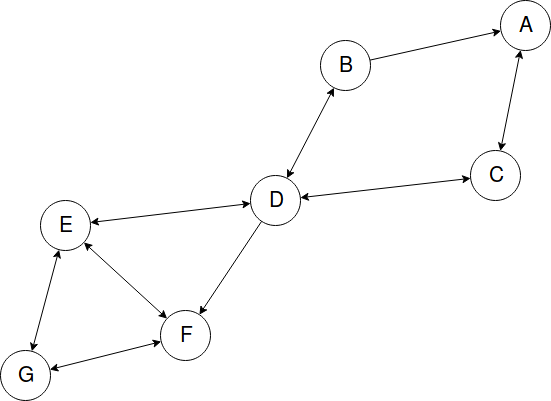
\includegraphics[scale=0.3]{../images/SampleConnectedGraph.png}
		\caption{A sample comparison graph with a total of 7 nodes. This graph is strongly connected as there exists a path using directed edges between any two nodes in the graph.}
		\label{fig:sub1}
	\end{subfigure}%
	\begin{subfigure}[t]{.45\textwidth}
		\centering
		\captionsetup{width=0.85\textwidth}
		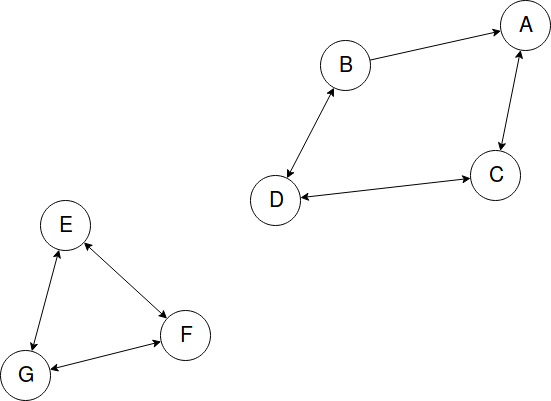
\includegraphics[scale=0.3]{../images/SampleDisconnectedGraph.png}
		\caption{A sample comparison graph with a total of 7 nodes. This graph is entirely disconnected as there exists disjoint subsets of nodes which have no connections between them.}
		\label{fig:sub2}
	\end{subfigure}%
	\label{fig}
\end{figure}

\subsection{Condition of Strong Connectivity}

The original constraint for paired-comparison data to be suitable for analysis such that all comparisons can be estimated was formulated by Ford in 1957 \cite{ford_1957}. This requirement originally stipulated that the comparison graph must be such that any node within the graph can be chosen and directed edges exists in such a way that movement along the existing edges admits a path to any other node in the graph. In graph theoretic terms, this condition is equivalent to \textbf{strong connectivity} or the comparison graph has the property of being \textbf{strongly connected}. It is important to note this is a stronger statement than an undirected graph being connected as the ``one-way streets'' formed by directed edges may not necessarily form a strongly connected graph. Figure Y shows an example of a directed graph which has an edge between all nodes but is not strongly connected. We will revisit the relationship between strong connectivity and undirected graphs shortly.

In order to evaluate the satisfaction of this assumption within a dataset of comparisons, we can use well known algorithms to determine the connectivity of the comparison graph. Tarjan's Algorithm by Robert Tarjan is an efficient algorithm which runs in linear time with regard to the number of nodes within a graph and determines the number of strongly connected components within a graph \cite{tarjan_1972}. Strongly connected components of a graph are disjoint subsets of nodes which are independently strongly connected despite the graph as a whole not being strongly connected. This algorithm can serve two purposes within the context of paired-comparison models. If the interest is in determining if the comparison graph is strongly connected, then the desired output from this algorithm is that the graph is constructed from one strongly connected component. However, in the event there exist more than one strongly-connected component within the graph (implying the entire graph is not strongly connected), the algorithm will return labels corresponding to disjoint sets of nodes which are strongly connected. In this case, a paired-comparison model can be fit to each of the strongly connected components identified, but comparisons across the strongly connected components will be unavailable. Figure Ya shows an example of a graph containing two strongly connected components while figure Xa shows an example of a being strongly connected.

\begin{figure}[!h]
	\centering
	\begin{subfigure}[t]{.45\textwidth}
		\centering
		\captionsetup{width=0.85\textwidth}
		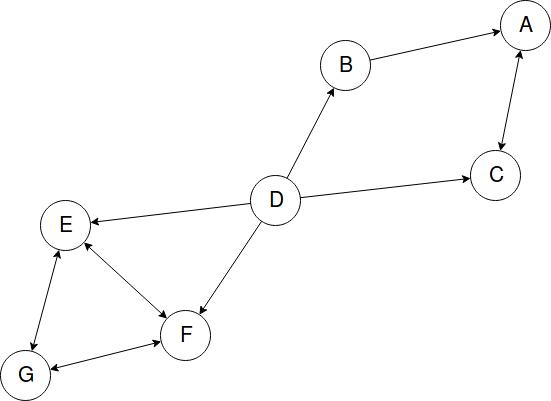
\includegraphics[scale=0.3]{../images/SampleWeaklyConnectedGraph.png}
		\caption{A comparison graph with a total of 7 nodes. This graph is weakly connected as there does not exist a path along directed edges between all nodes in the graph. Figure Yb shows the undirected edge connectivity of the graph. }
		\label{fig:sub1}
	\end{subfigure}%
	\begin{subfigure}[t]{.45\textwidth}
		\centering
		\captionsetup{width=0.85\textwidth}
		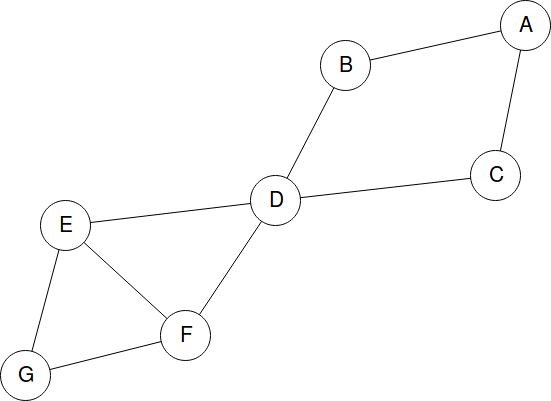
\includegraphics[scale=0.3]{../images/SampleUndirectedWeaklyConnectedGraph.png}
		\caption{A comparison graph with a total of 7 nodes. This graph is weakly connected as it is a transformation of the graph shown in Ya where each directional edge is replaced with a undirected or bidirectional edge. Using this transformation, there exists a path between any two nodes in the graph implying weak connectivity of the graph shown in Ya.}
		\label{fig:sub2}
	\end{subfigure}%
	\label{fig}
\end{figure}

\subsection{Condition of Weak Connectivity}

While strong connectivity of the comparison graph allows a paired-comparison model to be fit without issue, Yan (2014) discusses how using a singular pertubation method can allow for comparisons to be made when the graph is only \textbf{weakly connected.} Weakly connected graphs are directed graphs which, if transformed into an undirected graph and all directed edges are made undirected, the graph is connected (or all nodes can be reached from any other node). Figure Ya shows an example of a graph which is not strongly connected but is weakly connected. In Figure Ya, we see the original directed graph with node A having only directed edges away from it. However, if we remove the direction from each of the edges, we see in Figure Yb that the undirected version of this graph is connected. One intuitive reason for why weakly connected graphs are not sufficient without modification is that one team is undefeated and without an additional measure of "strength of win", the magnitude of how much the latent strength of this team differs from the next best team is unknown. Another intuitive reason is that node A in Figure Ya prevents the flow of information between strongly connected components. 

The singular pertubation method discussed by Yan is equivalent to adding a penalized term to the likelihood in such a way that a "pseudo-loss" to at least one other team is added to the comparison graph in order for the graph to become strongly connected.\cite{yan2016ranking} This term can be re-interpreted as a specific prior distribution to allow for the penalized term to exist within the likelihood.

% TODO: Discuss reformulation of likelihood

\subsection{Simulation of Graph Connectivity}

It is useful to understand how likely a graph is to be connected given some properties (number of nodes, number of edges). Assessing the probability of a graph being connected is a difficult combinatorial problem to solve analytically. However, it is possible to simulate the connectedness of a graph. In the case of the data we are analyzing, we assume that two characters are randomly chosen to participate in a match. This is a strong assumption about the underlying strucfture of how characters are chosen for a given match Specifically, it is unclear if SaltyBet uses any heuristic beyond randomness to choose characters for each match. This could be analyzed by attempting to determine if there are clusters of nodes within the graph which have a higher connectivity to other nodes. Unfortunately, the problem of detecting ``densely'' connected clusters within a graph is computational challenging as well and is beyond the scope of this project [CITE]. Instead, we will assume that of the 9,662 characters present, two characters are randomly chosen and then compared within a match. For our simulation, we will allow the order in which the characters are chosen to correspond to the direction of the edge between each character with the first character being chosen denoted as the winner of the match. This equates to 50\% win rate for each character. While this does not account for the underlying strength of a character, it provides a general enough framework for an intuition to be formed around how many matches are needed to be strongly connected. 

The simulation begins by generating 9,662 nodes and then randomly generating edges between them. The number of edges generated varies from 10,000 to 1,250,000 in steps of 500 with 50 simulated comparison graphs being generated at each step. We then apply Tarjan's Algorithm to determine the number of strongly connected components within each graph. In parallel to this experiment, we also measure the number of weakly connected components within each graph simulated and plot this information simultaneously. The results of this simulation are shown in Figure Z and Table A below.

The results of the simulation revealed that b

% TODO: Simulation Results (Figure)
% TODO: Simulation Results (Table)

% TODO: Summarize Simulation Results
% TODO: Mention code is available

\section{Data Analysis}

\subsection{Data Cleaning}

With the major components modeling, estimation, and diagnostic of this project discussed in detail, we begin to discuss the analysis of the SaltyBet data collected. First, we note some data cleaning steps. As discussed previously, SaltyBet consists of three phases: Matchmaking, Exhibition, and Tournament. Within the Exhibition mode teams of two characters are allowed to be requested by viewers. Since the data does not specify the makeup of each team, we remove matches which contain any team of characters. This accounts for only XYZ\% of the total number of matches. In addition, while ties are both permitted by SaltyBet and literature exists to incorporate this into the Bradley-Terry models, we remove them from this dataset for a number of reasons. First, ties are very unlikely within SaltyBet consisting of only XYZ\% of the data (XYZ matches). Second, if a tie does occur, it is typically due to either server failure or some unique attribute of the match up of characters (consider two identical characters being matched).

% TODO: Add percentage of team exhibition matches
% TODO: Add percentage of ties

\subsection{Exploratory Data Analysis}

After data cleaning, our data consists of a total of XYZ matches from a total of XYZ characters. Of all matches, XYZ characters have no losses with XYZ characters have no wins. The mean and median number of matches from each character is XYZ and XYZ, respectively. In addition, only XYZ\% have ever faced the same opponent twice. Of the characters who do face a repeat opponent, XYZ\% had at least one of the two matches requested in an exhibition match indicating that viewer intervention is the primary cause of repeat matches.

For hitbox data, the median hitbox height was XYZ pixels while the median hitbox width was XYZ pixels. Figure Z1 shows a density plot of each characters hitbox height and width. Of the XYZ characters within the cleaned dataset, XYZ\% fall within 10 pixels of the median height and width.

% TODO: Add percentage of team exhibition matches
% TODO: Total number of matches after data cleaning
% TODO: total number of characters after data cleaning
% TODO: total number of characters with no losses after data cleaning
% TODO: total number of characters with no wins after data cleaning
% TODO: mean number of matches from each character after data cleaning
% TODO: median number of matches from each character after data cleaning
% TODO: percent of characters who have faced repeat opponents
% TODO: percent of characters who have faced repeat opponents within exhibition mode



\nocite{*}

\newpage
\section{References - Left in for... reference}
\printbibliography

\newpage
\section{Appendix-R Code}
\singlespacing
\begin{lstlisting}
All that sweet sweet R code. 

Verbatim would also work here I think.

\end{lstlisting}
\end{document}

